%!TEX root = ../main.tex

\section{Теоретическое исследование: \\ анализ положений равновесия}
\label{sec:theoretical_analysis}

При определенных условиях электрический пробой может развиваться из малых возмущений свойств неповрежденной среды. Для отыскания этих условий исследуем положения равновесия уравнения \eqref{eq:one_dim} вида $\phi(x, t) \equiv C,$ $C \in [0, 1]$ (то есть $\phi$ постоянна и во времени, и в пространстве).

Приведем формулы для производных $f(\phi)$ и $\epsilon(\phi)$ (последняя задана выражением \eqref{eq:epsilon}):
\begin{gather*}
	f(\phi) = 4 \phi^3 - 3 \phi^4 \tsemicolon \quad f'(\phi) = 12 \phi^2 - 12 \phi^3 \tsemicolon \quad f''(\phi) = 24 \phi - 36 \phi^2 \tsemicolon \\
	\epsilon'_f = \cfrac{-\epsilon_0}{(f(\phi) + \delta)^2} \tsemicolon \quad \epsilon''_{ff} = \cfrac{2 \epsilon_0}{(f(\phi) + \delta)^3} \tsemicolon
\end{gather*}
откуда
\begin{gather}
	\epsilon'(\phi) = \epsilon'_f \cdot f' = \cfrac{-\epsilon_0 f'(\phi)}{(f(\phi) + \delta)^2} \tsemicolon
	\label{eq:epsilon_phi} \\
	\epsilon''(\phi) = \epsilon''_{ff} \cdot (f')^2 + \epsilon'_f \cdot f'' = \epsilon_0 \cfrac{2 (f'(\phi))^2 - f''(\phi)(f(\phi) + \delta)}{(f(\phi) + \delta)^3} \tpoint
	\label{eq:epsilon_phi_phi}
\end{gather}

Подставим решение $\phi(x, t) \equiv C$ в уравнение \eqref{eq:one_dim}, получим
\begin{equation}
	0 = \half K_\Phi^2 \epsilon'(C) + \cfrac{\Gamma}{l^2} f'(C) \tpoint
	\label{eq:equilibrium}
\end{equation}
Отсюда с учетом выражения \eqref{eq:epsilon_phi} имеем
$$f'(C) \left( \cfrac{\Gamma}{l^2} - \half K_\Phi^2 \cfrac{\epsilon_0}{(f(C) + \delta)^2} \right) = 0 \tpoint$$
Рассмотрим сначала случай $f'(C) = 0$: имеем $f'(C) = 12C^2 (1 - C) = 0$, следовательно, $C \in \{0, 1\}$. Значит, $\phi \equiv 0$ и $\phi \equiv 1$~-- положения равновесия.

Пусть теперь $C \neq 0, 1$. Тогда
$$\cfrac{\Gamma}{l^2} = \cfrac{K_\Phi^2 \epsilon_0}{2 (f(C) + \delta)^2} \quad \text{и} \quad f(C) + \delta = K_\Phi l \sqrt{\cfrac{\epsilon_0}{2 \Gamma}} \tpoint$$
Заметим, что $f(C) \in [0, 1]$, к тому же $f(\phi)$ строго возрастает, поэтому если $K_\Phi l \sqrt{\epsilon_0 / (2 \Gamma)} \in (\delta, 1 + \delta)$, то уравнение \eqref{eq:equilibrium} имеет отличный от $0$ и $1$ третий корень
\begin{equation}
	C_3 = f^{-1} \left( K_\Phi l \sqrt{\cfrac{\epsilon_0}{2 \Gamma}} - \delta \right) \tpoint
	\label{eq:equilibrium_third}
\end{equation}
В противном случае у уравнения \eqref{eq:equilibrium} корня только два.

Итак, число положений равновесия зависит от выполнения условия
\begin{equation}
	\delta^2 < \cfrac{K_\Phi^2 l^2 \epsilon_0}{2 \Gamma} < (1 + \delta)^2 \tpoint
	\label{cond:equilibriums_number}
\end{equation}
Немного позже станет ясна его связь со свойствами положений равновесия $\phi \equiv 0$ и $\phi \equiv 1$ и всего уравнения \eqref{eq:one_dim} в целом.

Перейдем теперь к анализу устойчивости положений равновесия.

Пусть $\phi(x, t)$~-- некоторое решение уравнения \eqref{eq:one_dim}, $\delta \phi(x, t)$~-- возмущение. Запишем уравнение \eqref{eq:one_dim} для возмущенного решения $\phi + \delta \phi$:
$$\cfrac{1}{m} \partt{(\phi + \delta \phi)} = \half K_\Phi^2 \epsilon'(\phi + \delta \phi) + \cfrac{\Gamma}{l^2} f'(\phi + \delta \phi) + \half \Gamma \partxx{(\phi + \delta \phi)} \tcomma$$
откуда
\begin{multline*}
	\cfrac{1}{m} \left( \partt{\phi} + \partt{(\delta \phi)} \right) = \half K_\Phi^2 [\epsilon'(\phi) + \epsilon''(\phi) \delta \phi + o(1) \delta \phi] + \\ + \cfrac{\Gamma}{l^2} [f'(\phi) + f''(\phi) \delta \phi + o(1) \delta \phi] + \half \Gamma \left( \partxx{\phi} + \partxx{(\delta \phi)} \right) \tpoint
\end{multline*}
С учетом того, что $\phi$~-- решение, перейдем к
$$\cfrac{1}{m} \partt{(\delta \phi)} = \half K_\Phi^2 [\epsilon''(\phi) + o(1)] \delta \phi + \cfrac{\Gamma}{l^2} [f''(\phi) + o(1)] \delta \phi + \half \Gamma \partxx{(\delta \phi)} \tpoint$$
Линеаризуем (отбросим бесконечно малые). Получим уравнение на возмущение
\begin{equation}
	\cfrac{1}{m} \partt{(\delta \phi)} = \left(\half K_\Phi^2 \epsilon''(\phi) + \cfrac{\Gamma}{l^2} f''(\phi) \right) \delta \phi + \half \Gamma \partxx{(\delta \phi)} \tpoint
	\label{eq:variation}
\end{equation}

Часть дальнейшего анализа удобно провести в общем виде, для уравнения
\begin{equation}
	\partt{(\delta \phi)} = A \delta \phi + B \partxx{(\delta \phi)} \tcomma
	\label{eq:variation_common}
\end{equation}
где $A$ и $B$~-- некоторые постоянные, причем $B > 0$.

Подставим в уравнение \eqref{eq:variation_common} $\delta \phi = e^{\alpha t} \sin(\omega x)$, то есть некоторую экспоненциально растущую или убывающую во времени (в зависимости от знака $\alpha$) гармонику, и получим уравнение относительно параметров возмущения
$$\alpha e^{\alpha t} \sin(\omega x) = A e^{\alpha t} \sin(\omega x) - B \omega^2 e^{\alpha t} \sin(\omega x) \tcomma$$
откуда
\begin{equation}
	\alpha = A - B \omega^2 \tpoint
	\label{eq:exponent_coefficient}
\end{equation}

Объединим три части рассуждения. Для уравнения \eqref{eq:one_dim} рассмотрим положение равновесия $\phi \equiv C$. Прибавим к нему возмущение $\delta \phi$; применим к~$\delta \phi$ уравнение \eqref{eq:variation}, в $\epsilon''$ и $f''$ подставим $\phi = C$. Полученное уравнение имеет вид~\eqref{eq:variation_common}. В зависимости от значения коэффициента
$$A = \half K_\Phi^2 \epsilon''(C) + \cfrac{\Gamma}{l^2} f''(C)$$
возможны три случая.
\begin{enumerate}[label=\arabic*.]
	\item $A > 0$. При $\omega^2 \in [0, A / B)$ верно $\alpha > 0$, то есть существуют возмущения $\delta \phi$, возрастающие во времени. Значит, положение равновесия $\phi \equiv C$ неустойчивое.
	\item $A < 0$. Для любого $\omega$ выполняется $\alpha \leqslant A < 0$. Любое возмущение $\delta \phi$ на отрезке $[0, W]_x$ можно представить в виде интеграла Фурье по гармоникам, все они убывают не медленнее гармоники $\omega = 0$. Значит, положение равновесия $\phi \equiv C$ устойчивое.
	\item $A = 0$. Рассуждаем аналогично случаю $A < 0$, однако здесь возможны сколь угодно медленно убывающие гармоники (со сколь угодно малым $\alpha$). Этот случай соответствует нейтральному равновесию. Здесь проведенного анализа с линеаризацией недостаточно; пояснение будет дано позже.
\end{enumerate}

Рассмотрим положение равновесия $\phi \equiv 0$. Имеем $f''(0) = 0, \; \epsilon''(0) = 0$ (см. выражение \eqref{eq:epsilon_phi_phi}); получаем $A = 0$. Этот случай требует более глубокого анализа, назвать тип положения равновесия мы пока не можем.

Рассмотрим положение равновесия $\phi \equiv 1$. Здесь $f''(0) = -12, \; \epsilon''(0) \hm = 12 \epsilon_0 / (1 + \delta)^2$ (см. выражение \eqref{eq:epsilon_phi_phi}); получаем
$$A = \half K_\Phi^2 \epsilon''(C) + \cfrac{\Gamma}{l^2} f''(C) = \cfrac{6 K_\Phi^2 \epsilon_0}{(1 + \delta)^2} - \cfrac{12 \Gamma}{l^2} \tpoint$$
Положение равновесия устойчиво при условии $A < 0$, то есть при
\begin{equation}
	\cfrac{K_\Phi^2 l^2 \epsilon_0}{2 \Gamma} < (1 + \delta)^2 \tpoint
	\label{cond:equilibrium_1_stable}
\end{equation}
Найдем $\omega_0$, при котором в случае неустойчивого положения равновесия возрастающие гармоники сменяются убывающими. Для этого рассмотрим выражение \eqref{eq:exponent_coefficient} с $\alpha = 0, \; B = \Gamma / 2$ и приведенным выше $A$. Получим
$$0 = \cfrac{6 K_\Phi^2 \epsilon_0}{(1 + \delta)^2} - \cfrac{12 \Gamma}{l^2} - \cfrac{\Gamma}{2} \omega_0^2 \tcomma$$
откуда
$$\omega_0 = 2 \sqrt{\cfrac{3 K_\Phi^2 \epsilon_0}{\Gamma (1 + \delta)^2} - \cfrac{6}{l^2}} \tpoint$$

Заметим, что условие \eqref{cond:equilibrium_1_stable} есть правое неравенство из условия \eqref{cond:equilibriums_number}. Чтобы объяснить это и сформировать полную картину происходящего, взглянем на положения равновесия немного под другим углом.

Решая уравнение \eqref{eq:equilibrium}, мы искали нули функции 
\begin{equation}
	\chi(\phi) = \half K_\Phi^2 \epsilon'(\phi) + \cfrac{\Gamma}{l^2} f'(\phi) \tpoint
	\label{eq:equilibruim_characteristic}
\end{equation}
Следовательно, любому положению равновесия $\phi \equiv C$ однозначно соответствует ноль~$C$ функции $\chi(\phi)$. Из вывода уравнения \eqref{eq:variation} на возмущение следует, что в его правой части при $\delta \phi$ стоит коэффициент $\chi'(\phi)$. После, проводя анализ уравнения \eqref{eq:variation_common} для положения равновесия $\phi \equiv C$, мы рассматривали случаи в зависимости от знака коэффициента $A$, который, как оказалось, равен $\chi'(C)$.

Подведем итог рассуждениям. Функция $\chi(\phi)$, определенная форму\forcehyphenation лой~\eqref{eq:equilibruim_characteristic}, гладкая на отрезке $[0, 1]$. Она имеет нули $0$ и $1$, а также при условии \eqref{cond:equilibriums_number}~-- третий ноль в некоторой точке $C_3 \in (0, 1)$. Положения равновесия $\phi \equiv C$ однозначно соответствуют нулям $\chi(\phi)$. Вопрос их устойчивости сводится к отысканию знака $\chi'(\phi)$ в нулях: положительная $\chi'$~-- неустойчивое равновесие, отрицательная $\chi'$~-- устойчивое.

Теперь стало понятно, почему в случае нулевой $\chi'$ (как в точке $\phi = 0$) недостаточно анализа с линеаризацией уравнения на возмущение. Интуитивно понятно, что в случае нулевой первой производной нужно рассмотреть первую ненулевую производную высшего порядка; возрастание $\chi$ будет означать неустойчивое равновесие, убывание~-- устойчивое.

В завершение докажем, что $\chi(\phi)$ в нуле $C_3 \in (0, 1)$ (в случае его существования) имеет ненулевую производную. Имеем
$$\chi(C_3) = f'(C_3) \left( \cfrac{\Gamma}{l^2} - \cfrac{K_\Phi^2 \epsilon_0}{2 (f(C_3) + \delta)^2} \right) = 0 \tpoint$$
Учитывая, что $f'(C_3) \ne 0$, получим
$$\cfrac{\Gamma}{l^2} - \cfrac{K_\Phi^2 \epsilon_0}{2 (f(C_3) + \delta)^2} = 0 \tpoint$$
Тогда
$$\chi'(\phi)|_{C_3} = f'(C_3) \left( \cfrac{\Gamma}{l^2} - \cfrac{K_\Phi^2 \epsilon_0}{2 (f(\phi) + \delta)^2} \right) ' \bigg|_{C_3} = (f'(C_3))^2 \cfrac{K_\Phi^2 \epsilon_0}{(f(C_3) + \delta)^3} \ne 0 \tpoint$$

Теперь можно провести исчерпывающий разбор случаев поведения $\chi(\phi)$ в своих нулях. Как видно из условий \eqref{cond:equilibriums_number} и \eqref{cond:equilibrium_1_stable}, оно определяется величиной
\begin{equation}
	\xi = \cfrac{K_\Phi^2 l^2 \epsilon_0}{2 \Gamma} \tpoint
	\label{char:equilibriums}
\end{equation}

Вначале рассмотрим случай $0 \leqslant \xi < \delta^2$. Нули $\chi(\phi)$: $0$, $1$; $\chi'(0) = 0, \; \chi'(1) \hm < 0$. Поведение функции $\chi(\phi)$ схематично изображено на рис. \ref{fig:equilibriums_case_1}. Положения равновесия: $\phi \equiv 0$ неустойчивое, $\phi \equiv 1$ устойчивое. Эту конфигурацию условно назовем случаем <<слабого электрического напряжения>>. Интуитивно конфигурация означает, что при фиксированных прочих параметрах электрическое поле мало настолько, что даже близкая к полностью разрушенной среда $\phi \approx 0$ со временем <<восстанавливается>> до $\phi \approx 1$.

Рассмотрим теперь случай $\delta^2 < \xi < (1 + \delta)^2$. Нули $\chi(\phi)$: $0$, $C_3$ (см. выражение~\eqref{eq:equilibrium_third}), $1$; $\chi'(0) = 0, \; \chi'(1) < 0; \; \chi'(C_3) > 0$ (из гладкости $\chi$). Поведение функции $\chi(\phi)$ схематично изображено на рис. \ref{fig:equilibriums_case_2}. Положения равновесия: $\phi \equiv 0$ устойчивое, $\phi \equiv C_3$ неустойчивое, $\phi \equiv 1$ устойчивое. Такую конфигурацию условно назовем случаем <<среднего электрического напряжения>>. Интуитивно конфигурация означает, что при достаточно близких к $0$ значениях $\phi$ среда <<разрушается>> до $0$, при достаточно близких к $1$~-- <<восстанавливается>> до $1$; посередине же, <<на границе>>,~-- неустойчивое равновесие.

Наконец, рассмотрим случай $(1 + \delta)^2 < \xi$. Нули $\chi(\phi)$: $0$, $1$; $\chi'(0) = 0,$ $\chi'(1) > 0$. Поведение функции $\chi(\phi)$ схематично изображено на рис. \ref{fig:equilibriums_case_3}. Положения равновесия: $\phi \equiv 0$ устойчивое, $\phi \equiv 1$ неустойчивое. Эту конфигурацию условно назовем случаем <<сильного электрического напряжения>>. Интуитивно конфигурация означает, что электрическое поле достаточно сильно, чтобы сколь угодно близкую к неповрежденной среду $\phi \approx 1$ <<разрушить>> до $\phi \approx 0$. Именно в этом случае электрический пробой развивается из малых возмущений свойств неповрежденной среды.

Во всех трех случаях устойчивость положения равновесия $\phi \equiv 0$ определяется по производной высшего порядка из вида функции $\chi(\phi)$.

\begin{figure}[!tp]
	\centering
	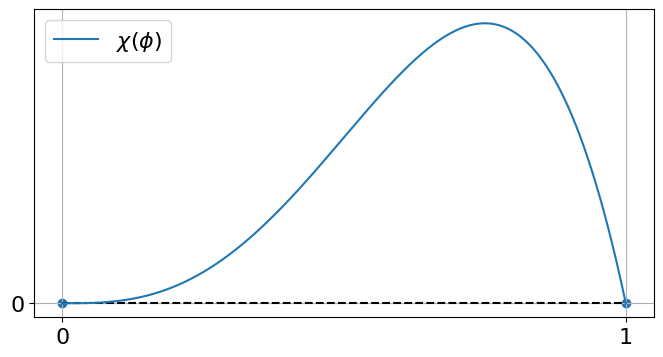
\includegraphics[width=0.77\textwidth]{figures/equilibriums_case_1.png}
	\vspace{-0.3cm}
	\caption{Поведение функции $\chi(\phi)$, случай <<слабого напряжения>>}
	\label{fig:equilibriums_case_1}
	\vspace{0.7cm}
	
	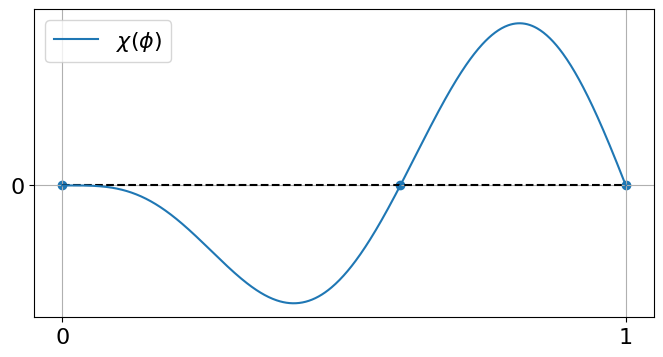
\includegraphics[width=0.77\textwidth]{figures/equilibriums_case_2.png}
	\vspace{-0.3cm}
	\caption{Поведение функции $\chi(\phi)$, случай <<среднего напряжения>>}
	\label{fig:equilibriums_case_2}
	\vspace{0.7cm}
	
	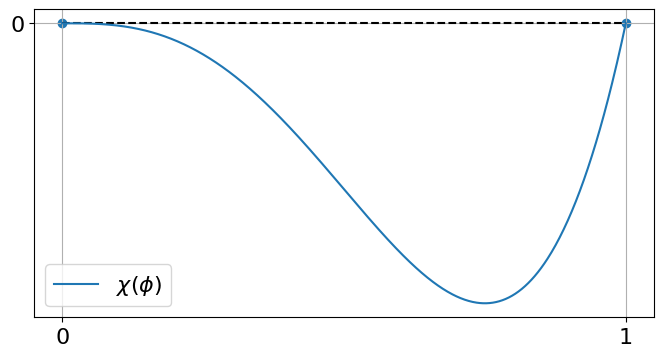
\includegraphics[width=0.77\textwidth]{figures/equilibriums_case_3.png}
	\vspace{-0.3cm}
	\caption{Поведение функции $\chi(\phi)$, случай <<сильного напряжения>>}
	\label{fig:equilibriums_case_3}
\end{figure}